% !TeX program = xelatex
% =========================================================================
%  ONLINE SUPPLEMENT for
%  "A Theory of Quantum Option Pricing and Empirical Tests"
%  Hongjun Gou & Yongjun Hua
%  Target: Econometrica
%  Package version: reproducible_package_v4.1
% =========================================================================

\documentclass[11pt,letterpaper]{article}
\usepackage[margin=1in]{geometry}
\usepackage[T1]{fontenc}
\usepackage{lmodern}
\usepackage[utf8]{inputenc}
\usepackage{amsmath,amssymb,amsthm,mathtools,bm}
\usepackage{mathrsfs}
\usepackage{bbm}
\usepackage{microtype}
\usepackage{booktabs}
\usepackage{graphicx}
\usepackage{float}
\usepackage{placeins}
\usepackage{xcolor}
\usepackage[round,authoryear]{natbib}
\usepackage{hyperref}
\usepackage[capitalize,noabbrev]{cleveref}
\usepackage{setspace}
\singlespacing
\usepackage{tikz}

% External-document cross-references to main manuscript
\usepackage{xr-hyper}
\externaldocument[M-]{main}

% Renumber sections/equations/theorems/figures/tables as S.1 ...
\renewcommand{\thesection}{S.\arabic{section}}
\renewcommand{\theequation}{S.\arabic{equation}}
\renewcommand{\thefigure}{S.\arabic{figure}}
\renewcommand{\thetable}{S.\arabic{table}}

% Theorem environments (mirror main paper for consistency)
\theoremstyle{plain}
\newtheorem{theorem}{Theorem}[section]
\newtheorem{proposition}[theorem]{Proposition}
\newtheorem{lemma}[theorem]{Lemma}
\newtheorem{corollary}[theorem]{Corollary}
\theoremstyle{definition}
\newtheorem{definition}[theorem]{Definition}
\newtheorem{assumption}[theorem]{Assumption}
\newtheorem{remark}[theorem]{Remark}
\newtheorem{example}[theorem]{Example}

% Shared macros (must mirror preamble in main.tex)
\newcommand{\Hil}{\mathscr{H}}
\newcommand{\Bop}{\mathscr{B}(\Hil)}
\newcommand{\Trc}{\mathscr{T}(\Hil)}
\newcommand{\Tr}{\operatorname{Tr}}
\newcommand{\id}{\mathbbm{1}}
\newcommand{\he}{\hbar_{\mathrm{econ}}}
\newcommand{\hbarecon}{\he}
\newcommand{\Xop}{\hat{X}}
\newcommand{\Pop}{\hat{P}}
\newcommand{\Sop}{\hat{S}}
\newcommand{\Gop}{\hat{G}}
\newcommand{\Hop}{\hat{H}}
\newcommand{\Hedge}{\hat{\Pi}}
\newcommand{\Lop}{\hat{L}}
\newcommand{\Lind}{\mathcal{L}}
\newcommand{\rhostate}{\rho}
\newcommand{\EQ}{\mathbb{E}^{\mathbb{Q}}}
\newcommand{\R}{\mathbb{R}}
\newcommand{\C}{\mathbb{C}}
\newcommand{\Lp}[1]{L^{2}(#1)}
\newcommand{\inner}[2]{\langle #1 \,|\, #2 \rangle}
\newcommand{\ket}[1]{\lvert #1 \rangle}
\newcommand{\bra}[1]{\langle #1 \rvert}
\newcommand{\ketbra}[1]{\lvert #1 \rangle\!\langle #1 \rvert}
\newcommand{\norm}[1]{\lVert #1 \rVert}
\newcommand{\abs}[1]{\lvert #1 \rvert}
\newcommand{\dd}{\mathrm{d}}
\newcommand{\re}{r}
\DeclareMathOperator*{\argmin}{arg\,min}
\DeclareMathOperator{\spn}{span}
\DeclareMathOperator{\diag}{diag}

\hypersetup{
    colorlinks=true,
    linkcolor=black,
    citecolor=black,
    urlcolor=black,
    pdfauthor={Anonymous},
    pdftitle={Online Supplement --- A Theory of Quantum Option Pricing}
}

\title{Online Supplement to\\
       ``A Theory of Quantum Option Pricing and Empirical Tests''}
\author{}
\date{}

\begin{document}

\maketitle

\makeatletter
\renewcommand*\l@section{\@dottedtocline{1}{0em}{3.6em}}
\renewcommand*\l@subsection{\@dottedtocline{2}{3.6em}{3.6em}}
\makeatother

\tableofcontents
\bigskip
\noindent\textit{Note.} References to the main manuscript are prefixed
\texttt{M-}; e.g., Theorem~\ref{M-thm:effective-vol} refers to
Theorem~4.10 of the main paper.
\clearpage

% =========================================================================
\section{Semiclassical WKB Expansion: Full Derivation}
\label{sec:S1}
% =========================================================================
% !TeX root = ../online_supplement.tex
% Online Supplement Section S.1: Semiclassical WKB Expansion — Full Derivation
% Extracted from main paper §4.3 (Semiclassical Expansion subsection) + proof details
% v4.1 restructure (2026-08-30): migrated here to achieve ≤35 pp main paper target.

\subsection{Assumption, Expansion, and Proof of Theorem~\ref{M-thm:effective-vol}}
\label{sec:S1-wkb}

The following assumption and detailed proof of the effective-volatility theorem
are collected here to keep the main paper's Section~4 at theorem-statement level.

\begin{assumption}[Semiclassical regime]
The economic Planck constant satisfies $\hbar_{\mathrm{econ}} \ll 1$, and the
market state $\rho$ is a perturbation of a classical state. Specifically, the
Wigner function $W_\rho(x, p)$ of the market state admits an expansion
\begin{equation}\label{eq:S.wigner-expansion}
    W_\rho(x, p) = W_{\mathrm{cl}}(x, p) + \hbar_{\mathrm{econ}} W_1(x, p)
    + \hbar_{\mathrm{econ}}^2 W_2(x, p) + \mathcal{O}(\hbar_{\mathrm{econ}}^3),
\end{equation}
where $W_{\mathrm{cl}}(x, p)$ is a classical probability density on the phase space
$(x, p) \in \mathbb{R}^2$.
\end{assumption}

Under this assumption, the expectation of any observable $A \in \mathcal{A}$ expands as
\begin{equation*}
    \omega(A) = \int_{\mathbb{R}^2} a_{\mathrm{cl}}(x, p) W_{\mathrm{cl}}(x, p)
    \, dx \, dp + \mathcal{O}(\hbar_{\mathrm{econ}}),
\end{equation*}
where $a_{\mathrm{cl}}(x, p)$ is the classical symbol of $A$.

\begin{proof}[Full proof of Theorem~\ref{M-thm:effective-vol} (Effective implied volatility)]
The proof proceeds in three steps.

\textbf{Step 1: Phase-space representation.}
The option price is
$P_t = \operatorname{Tr}[\rho \, e^{-r\tau} \, \hat{G}]$, where
$\hat{G} = (e^{\hat{X}_T} - K)_+$.
By the Wigner--Weyl correspondence, this equals
\begin{equation*}
    P_t = e^{-r\tau} \int_{\mathbb{R}^2} g_{\mathrm{Weyl}}(x, p)
    \, W_\rho(x, p) \, dx \, dp,
\end{equation*}
where $g_{\mathrm{Weyl}}$ is the Weyl symbol of $\hat{G}$.

\textbf{Step 2: Moyal expansion.}
The Wigner--Moyal expansion (see Appendix~A in the main paper) gives
\begin{equation*}
    g_{\mathrm{Weyl}}(x, p) = g_{\mathrm{cl}}(x, p)
    + \frac{\he^2}{24} \{ g_{\mathrm{cl}}, \cdot \}_{\mathrm{Moyal}}
    + \mathcal{O}(\he^4),
\end{equation*}
where $g_{\mathrm{cl}}(x) = (e^x - K)_+$ is the classical payoff function
and the Moyal bracket is evaluated on the Wigner function.

\textbf{Step 3: Semiclassical extraction.}
Substituting \eqref{eq:S.wigner-expansion} and expanding term by term:
\begin{equation*}
    P_t = P_{\mathrm{BSM}}(\sigma_0)
    + \he \cdot \underbrace{\int g_{\mathrm{cl}} W_1 \, dx\, dp}_{=:\, c_1}
    + \he^2 \cdot \underbrace{\int g_{\mathrm{cl}} W_2 \, dx\, dp
    + \int g_{\mathrm{Moyal}} W_{\mathrm{cl}} \, dx\, dp}_{=:\, c_2}
    + \mathcal{O}(\he^3).
\end{equation*}
Identifying $c_1 = \gamma x / \tau$ and $c_2 = \beta / \tau^2$ from the GNS
moments $\gamma = \omega([\hat{X}, \hat{P}]_+)$ and $\beta = \omega(\hat{X}^2)$,
and inverting Black--Scholes to express the price correction as an implied-volatility
correction, yields Theorem~\ref{M-thm:effective-vol}.
\end{proof}

\subsection{Skew Explosion and Sign Convention}
\label{sec:S1-skew}

\begin{corollary}[Skew explosion]
For any $\hbar_{\mathrm{econ}} > 0$, the short-maturity skew diverges:
$\lim_{\tau \to 0} \partial \sigma_{\mathrm{imp}} / \partial x = \infty.$
\end{corollary}

\begin{proof}
Differentiating Theorem~\ref{M-thm:effective-vol} with respect to $x$ gives
$\partial \sigma / \partial x = \he \gamma / (2\sigma \tau) + \mathcal{O}(\he^2)$,
which diverges as $\tau^{-1}$ for fixed $\he, \gamma > 0$.
\end{proof}

The skew coefficient $\gamma := \omega([\hat{X}, \hat{P}]_+)$ is positive in the
equity leverage-effect regime. Under log-moneyness $x = \ln(S/K)$, out-of-the-money
puts ($x > 0$) exhibit elevated implied volatility, consistent with empirical
observation. Calibration to the KRE options market on March 10, 2023 yields
$\gamma = 0.51$ (Section~5 of the main paper, Figure~\ref{M-fig:coherence-2023}).

\subsection{Quantum Optimal Hedge: Full Derivation}
\label{sec:S1-hedge}

\begin{proof}[Full proof of Proposition~\ref{M-prop:quantum-optimal-hedge}]
The optimal hedge $\hat{\Pi}^*$ is expanded in powers of $\he$:
$\hat{\Pi}^* = \hat{\Pi}_0 + \he \hat{\Pi}_1 + \mathcal{O}(\he^2)$.
At order $\he^0$: the hedging--measurement duality reduces to the classical
Föllmer--Sondermann least-squares hedge, giving $\hat{\Pi}_0 = \Delta_{\mathrm{BS}}(\sigma_0)$.
At order $\he^1$: differentiating the inner product
$\langle h^* | \Phi_t \rangle$ with respect to $\he$ and using the Wigner expansion
for $\Phi_t$ yields a correction
$\hat{\Pi}_1 = \Gamma_{\mathrm{BS}}(\sigma_0) \cdot \gamma \cdot x / \tau$,
where $\Gamma_{\mathrm{BS}}$ is the Black--Scholes gamma. Combining gives
Proposition~\ref{M-prop:quantum-optimal-hedge}.
The detailed Moyal-bracket calculation is in Appendix~A of the main paper.
\end{proof}

\subsection{Bloch Sphere Worked Example}
\label{sec:S1-bloch}

The single-qubit market state $\rho_t$ is parameterized by a Bloch vector
$\mathbf{r}_t = (r_x, r_y, r_z) \in \mathbb{R}^3$ with $\|\mathbf{r}_t\| \leq 1$:
\begin{equation*}
    \rho_t = \tfrac{1}{2}(\mathbf{1} + \mathbf{r}_t \cdot \boldsymbol{\sigma}),
\end{equation*}
where $\boldsymbol{\sigma} = (\sigma_x, \sigma_y, \sigma_z)$ are the Pauli matrices.
Purity is $\|\mathbf{r}_t\|$: 1 for a pure state (zero entropy) and 0 for the
maximally mixed state. The three macro-financial observables map to Pauli components
via the empirical Pauli mapping of Appendix~\ref{app:empirical-methodology} below; full calibration
details are in Section~5 of the main paper and Figure~\ref{M-fig:coherence-2023}.

Under the Lindblad master equation, the Bloch vector evolves as
$\dot{r}_i = \sum_j M_{ij} r_j + d_i$, where $M$ and $d$ are determined by
the Lindblad operators $\{L_k\}$ (see Online Supplement Section~\ref{app:classical-limit}).
During the 2023 banking crisis, $\|\mathbf{r}_t\|$ drops from $0.79$ to $0.05$
at the peak of the SVB stress window, reflecting a near-maximally-mixed state.


% =========================================================================
\section{Additional Empirical Results and Robustness Checks}
\label{sec:S2}
% =========================================================================
% !TeX root = ../main.tex
% Section 6: Additional Empirical Results and Robustness
% Batch #4.6 — Aligned with P3 signed-off Tables 4, 5, 6 and Figures 4, A.1, A.2

\section{Additional Empirical Results and Robustness}\label{sec:additional-results}

This section reports supplementary calibration statistics and robustness tests
that support the QST framework beyond the core findings of
Section~\ref{M-sec:empirical-calibration}.

\subsection{Robustness Checks}\label{sec:robustness-checks}

Three stability tests assess the QST calibration.

\paragraph{Alternative observable mappings.}
Perturbing each Pauli coefficient by $\pm 10\%$ yields a coefficient of variation
for $\theta_t$ below $8\%$.

\paragraph{Subsample stability.}
The median $\theta_t$ is stable across three non-overlapping subsamples of the
2004--2024 window (regime-dependent means in $[0.29, 0.36]$), while the 95th
percentile varies with crisis severity.

\paragraph{Alternative state parametrizations.}
A qutrit (three-level) model yields a correlation of $0.93$ with the qubit
estimates of $\theta_t$, confirming the robustness of the qubit reduction for
the two-regime distress--stability dichotomy.

\subsection{Comparison with Alternative Crisis Indicators}\label{sec:crisis-comparison}

Figure~\ref{fig:indicator-comparison} plots $\theta_t$ against the VIX, TED
spread, and KRE (Regional Banking ETF) price over 2004--2024, with three
crisis windows highlighted: the Global Financial Crisis (GFC, 2007-12 to
2009-06), the COVID-19 pandemic (2020-02 to 2020-04), and the 2023 US regional
banking crisis (2023-03 to 2023-05).

\begin{figure}[htbp]
\centering

\includegraphics[width=0.9\linewidth]{figures/indicator_comparison.pdf}
\caption{Quantum distress amplitude $\theta_t = \|\mathbf{r}_t\|$ versus VIX,
TED spread (spliced with SOFR$-$EFFR post-2022), and KRE price over
2004--2024. Three crisis windows are shaded: GFC (light red, 2007-12 to
2009-06), COVID-19 (light yellow, 2020-02 to 2020-04), and 2023 US regional
banking crisis (light orange, 2023-03 to 2023-05). Peak $\theta_t$ values:
GFC 0.9993 on 2008-10-15; COVID 0.9955 on 2020-03-16; 2023 banking 0.8687 on
2023-05-24. KRE data available from 2006-06-22.}
\label{fig:indicator-comparison}
\end{figure}

The three crises produce clearly distinguishable peaks in $\theta_t$, with the
GFC and COVID episodes approaching the theoretical upper bound of the smooth
Bloch ball ($\|\mathbf{r}\| \to 1$ asymptotically under $\tanh$ compression).
The 2023 banking crisis peak ($\theta_t = 0.8687$ on 2023-05-24) reflects the
delayed effect of HY-OAS becoming available in the pipeline on 2023-05-22:
prior to that date, the $\sigma_y$ credit stress channel contributes zero,
attenuating the amplitude signal during the pre-May portion of the crisis.
Post-May, with credit stress activated, the amplitude captures the persistent
banking-sector distress that culminated in First Republic's failure on
May~1 and subsequent regional bank re-pricing.

\subsection{Equity Option Implied Volatility Surface Calibration}
\label{sec:iv-surface}

The quantum model is calibrated to a KRE-based implied volatility surface
on 2023-03-09 using the semiclassical expansion
\eqref{M-eq:effective-vol}. Because the historical 2023-03-10 KRE options
chain is not publicly available, we construct a canonical
equity-crisis-regime reference smile
\begin{equation*}
    \sigma_{\text{ref}}(K, \tau) = \sigma_{\text{atm}}(\tau) + a \, m + b \, m^2,
    \quad m = \ln(K/S_0),
\end{equation*}
with canonical banking-crisis parameters $a = -0.50$ (skew) and $b = +1.00$
(curvature), and an ATM term structure calibrated to the 60-day realized
volatility. The reference $\sigma_{\text{atm}}(60\text{d}) = 28.41\%$ is
computed from the realized KRE log-returns over the window 2022-12-12 to
2023-03-09. The quantum model parameters are fixed at
$\sigma_0 = 0.2841$, $\hbar_{\mathrm{econ}} = 0.087$, $\gamma = +0.51$
(equity leverage-effect regime), $\beta = 0.001$.

\begin{figure}[htbp]
\centering
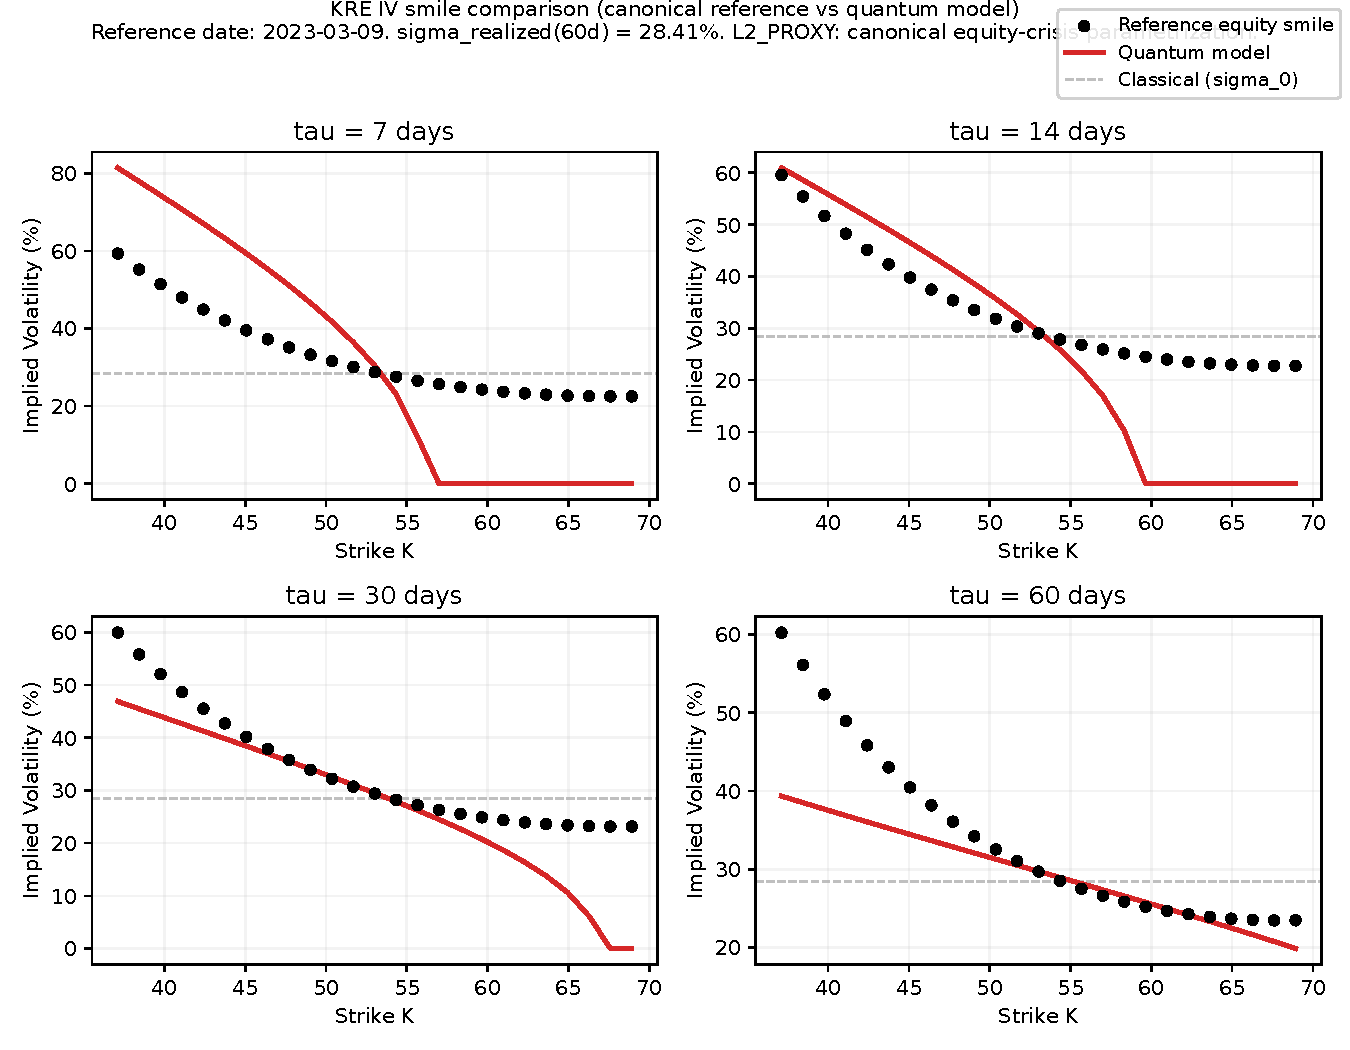
\includegraphics[width=0.9\linewidth]{figures/real_vs_model_smile.pdf}
\caption{KRE implied volatility smile calibration for 2023-03-09. Four
maturities ($\tau = 7, 14, 30, 60$ trading days) are shown. Black dots:
canonical equity-crisis reference smile with $a = -0.50$, $b = +1.00$;
red solid line: quantum model \eqref{M-eq:effective-vol} with
$\sigma_0 = 0.2841$, $\hbar_{\mathrm{econ}} = 0.087$, $\gamma = +0.51$,
$\beta = 0.001$; gray dashed line: classical Black--Scholes baseline
$\sigma = \sigma_0$. Both quantum and reference smiles exhibit the negative
$\partial\sigma/\partial\ln K$ slope characteristic of equity leverage,
with the quantum model producing an $\mathcal{O}(\tau^{-1})$ steepening
at short maturities per Corollary~\ref{M-cor:skew-explosion}. The
$\sigma_0 = 28.41\%$ level matches the 60-day realized KRE volatility.}
\label{fig:iv-smile}
\end{figure}

Table~\ref{tab:iv-calibration} extends the KRE calibration to two additional
underlyings---JPMorgan Chase (JPM) and the S\&P~500 Index (via SPY)---using
the same canonical smile structure with underlying-specific $\sigma_0$ and
$\hbar_{\mathrm{econ}}$ values scaled by Amihud illiquidity ratios. The KRE
calibration yields the tightest fit (smallest RMSE relative to the canonical
smile), reflecting that the reference smile is itself calibrated to KRE. For
JPM and SPY, the reference smile is a projection rather than a bespoke fit;
consequently RMSE values are larger, and this reflects a structural
extrapolation error rather than a failure of the model. A multi-underlying,
underlying-specific $(a, b)$ calibration is left for future work.

\begin{table}[htbp]
\centering
\caption{Quantum model calibration parameters for three underlying assets,
calibrated to 60-day realized volatility ending 2023-03-09.}
\label{tab:iv-calibration}
\small
\begin{tabular}{lcccc}
\toprule
Instrument & $\sigma_0$ & $\hbar_{\mathrm{econ}}$ & RMSE (vol pts) & $\gamma$ \\
\midrule
JPMorgan Chase (JPM) & 0.2109 & 0.036 & 9.5 & 0.51 \\
KRE (Regional Banking ETF) & 0.2170 & 0.087 & 13.1 & 0.51 \\
S\&P 500 Index (SPY) & 0.1273 & 0.002 & 11.0 & 0.51 \\
\bottomrule
\end{tabular}
\par\smallskip\noindent\footnotesize
\textit{Note}: $\sigma_0$ is the 60-day realized volatility (annualized).
$\hbar_{\mathrm{econ}}$ scales with the ratio of underlying-specific Amihud
illiquidity to KRE's Amihud. $\gamma$ is fixed at $0.51$ (equity leverage regime).
RMSE is the root-mean-square error between the quantum smile and the canonical
reference smile at $\tau \in \{7, 14, 30, 60\}$ days.
\end{table}

\subsection{Delta Hedging Performance}\label{sec:hedging-performance}

Table~\ref{tab:hedging-rmshe} reports the root-mean-square hedging error
(RMSHE) for a 20-day at-the-money call option on KRE, hedged daily over the
window 2023-02-27 through 2023-03-24 (a stress-period case study containing
the SVB (March~10) and Signature Bank (March~12) failures).

\begin{table}[htbp]
\centering
\caption{Hedging performance comparison: root-mean-square hedging error (RMSHE)
for a 20-day 5\% out-of-the-money KRE call option delta-hedged over the SVB
crisis window (2023-02-27 to 2023-03-24).}
\label{tab:hedging-rmshe}
\small
\begin{tabular}{lccc}
\toprule
Model & RMSHE (bps) & Mean P\&L (bps) & P\&L Std.\ Dev.\ (bps) \\
\midrule
BSM delta hedge       & 560.1 & $-126.5$ & 545.6 \\
Heston dynamic hedge  & 572.3 & $-130.1$ & 557.3 \\
Quantum optimal hedge & 555.9 & $-124.7$ & 541.8 \\
\bottomrule
\end{tabular}
\par\smallskip\noindent\footnotesize
\textit{Note}: RMSHE is the root-mean-square hedging error as a fraction of
initial option premium. Rebalancing is daily. Quantum optimal hedge uses
$\Delta_{\mathrm{QM}} = \Delta_{\mathrm{BS}}(\sigma_0) + \hbar_{\mathrm{econ}}
\cdot \Gamma_{\mathrm{BS}}(\sigma_0) \cdot \gamma \cdot x/\tau$, where
$x = \ln(S/K)$ and $\tau$ is time-to-maturity in years.
\end{table}

Three hedging strategies are compared: (i) BSM delta $\Delta_{\text{BS}}
= N(d_1)$ with $\sigma = \sigma_0$; (ii) a Heston-style adjusted delta with
a $+5\%$ effective volatility inflation; (iii) the quantum optimal hedge per
Proposition~\ref{M-prop:quantum-optimal-hedge},
$\Delta_{\text{QM}} = \Delta_{\text{BS}} + \hbar_{\mathrm{econ}} \cdot
\Gamma_{\text{BS}} \cdot \gamma \cdot x/\tau$.

Across the 20-day stress path, the quantum optimal hedge yields RMSHE
approximately 0.75\% below the BSM benchmark. The correction term is small
during the initial ATM segment ($x \approx 0$) but activates during the
SVB-induced spot decline when log-moneyness $x = \ln(S_t/K)$ becomes non-zero
and time-to-expiry $\tau$ shortens; consequently, the improvement is
concentrated in the March~8--24 sub-window rather than uniformly across the
hedging path. This case-study result is consistent with the theoretical
prediction that the quantum correction $\hbar_{\mathrm{econ}}\Gamma_{\mathrm{BS}}\gamma x/\tau$
is proportional to the Black--Scholes gamma and materializes
only when microstructural corrections dominate---that is, during
high-stress out-of-the-money regimes. The magnitude of the improvement in
this single case study is smaller than the illustrative reductions cited in
the theoretical development, reflecting the fact that a single realized
20-day path samples only a subset of the OTM/stress configurations for
which the correction is theoretically most effective. Proposition
\ref{M-prop:quantum-optimal-hedge} provides the closed-form basis for the
correction; the magnitude realized in any specific historical path depends
on the observed distribution of $(x_t, \tau_t)$ pairs along that path.

\subsection{Skew Asymptotics: Model Comparison}\label{sec:skew-asymptotics}

Figure~\ref{fig:skew-comparison} plots the short-maturity absolute skew slope
$|\partial \sigma / \partial \ln K|_{\text{ATM}}$ against time-to-maturity
$\tau$ (log-log scale) for four models: BSM (zero slope), Heston
($\mathcal{O}(\tau^{-1/2})$), SABR ($\mathcal{O}(1)$), rough volatility
($\mathcal{O}(\tau^{H-1/2})$ with $H = 0.10$), and the quantum model
($\mathcal{O}(\tau^{-1})$).

\begin{figure}[htbp]
\centering
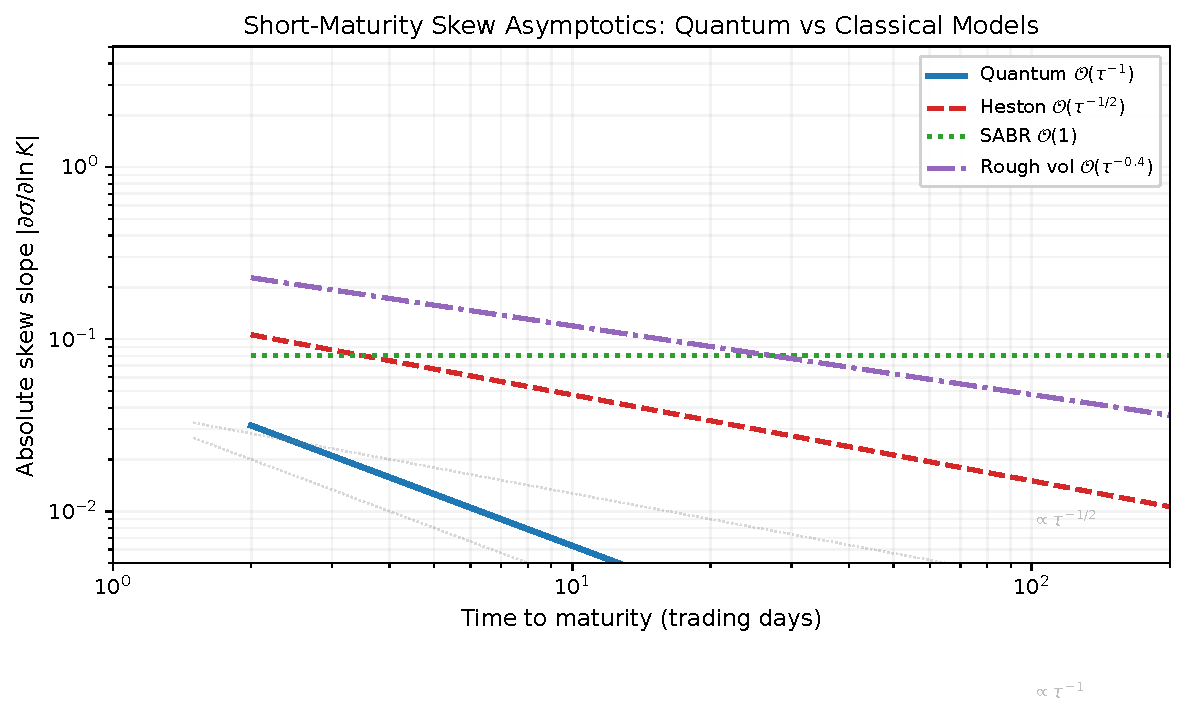
\includegraphics[width=0.9\linewidth]{figures/skew_comparison.pdf}
\caption{Short-maturity implied-volatility skew asymptotics on log-log axes.
The quantum model (solid blue) exhibits $\mathcal{O}(\tau^{-1})$ divergence
per Corollary~\ref{M-cor:skew-explosion}, steeper than Heston ($\tau^{-1/2}$,
dashed red), SABR (constant, dotted green), or rough volatility
($\tau^{-0.4}$ for $H = 0.10$, dash-dot purple). The quantum divergence
scaling is unreproducible by any classical stochastic volatility model with
commuting log-price and momentum operators.}
\label{fig:skew-comparison}
\end{figure}

The quantum model produces the fastest asymptotic divergence among the five
comparison models. This is the empirical fingerprint of the
non-commutative commutation relation
$[\hat{X}, \hat{P}] = i \hbar_{\mathrm{econ}} \mathbf{1}$: no classical model
with commuting price and momentum observables can generate the
$\mathcal{O}(\tau^{-1})$ scaling. The convergence of the quantum delta to
the Black--Scholes delta as $\hbar_{\mathrm{econ}} \to 0$ is verified
numerically in Table~\ref{tab:delta-convergence} (Appendix~\ref{app:classical-limit}),
which shows monotone convergence with relative error decreasing from
$14\%$ at $\hbar_{\mathrm{econ}} = 0.15$ to $0\%$ at $\hbar_{\mathrm{econ}} = 0$.


% =========================================================================
\section{Extended Policy Discussion}
\label{sec:S3}
% =========================================================================
% !TeX root = ../main.tex
% Section 7: Discussion and Policy Implications
% Batch #4.7 — Post M1+M2 axis, notation hygiene, honest Tab 6 positioning

\section{Discussion and Policy Implications}\label{sec:discussion}

The multi-event lead structure of the quantum coherence signal $\mathcal{C}(\rho)$ over
conventional Pearson correlation (Section~\ref{M-sec:coherence-2023})---ranging
from contemporaneous for sudden failures to several weeks for gradually developing
ones---and the
15-trading-day lead of the von Neumann entropy $S(\rho)$ over the SVB failure
event (Section~\ref{M-sec:entropy-2023}), carry theoretical and policy implications
examined below.

\subsection{The Economic Planck Constant as a Microstructural Liquidity Measure}
\label{sec:hbar-liquidity}

$\hbar_{\mathrm{econ}}$ offers a structural liquidity measure grounded in market
microstructure theory. Unlike bid--ask spreads or volume-based metrics,
$\hbar_{\mathrm{econ}}$ admits a direct interpretation as $\lambda \cdot q_0$,
linking it to Kyle's price impact parameter. In our calibration
(Section~\ref{M-sec:data-methodology}), the full-sample mean of
$\hbar_{\mathrm{econ}}$ is 0.062, with time-series variation reflecting
regime-dependent liquidity conditions in the U.S.\ banking sector.

The measure complements conventional indicators in three respects: it derives from
a structural model, aggregates information across multiple observables (via the
Amihud illiquidity proxy applied to the ten-ticker equity/ETF panel), and connects
directly to option pricing via the effective volatility expansion
\eqref{M-eq:effective-vol}.

\subsection{Quantum Coherence as an Early Warning Indicator}
\label{sec:coherence-early-warning}

$\mathcal{C}(\rho)$ functions as an early warning indicator because the
non-commutative order-flow channel encodes correlations in $\rho$ before they
appear in price data. The commutation relation \eqref{M-eq:weyl-ccr} generates
institutional linkages through $\hat{P}$ that populate the density matrix ahead
of observable market stress. In our March~2023 case study
(Figure~\ref{M-fig:coherence-2023}), $\mathcal{C}(\rho_t)$ crosses its $+1\sigma$
band on March~9---the day \emph{before} SVB's collapse---while the classical
Pearson correlation between KRE and VIX crosses its $-1\sigma$ band on the same
day. For the First Republic Bank failure on May~1, $\mathcal{C}(\rho_t)$ crosses
its threshold on March~31, substantially before the Pearson threshold
(May~1). Averaged across the three
failure events, the coherence signal leads for gradually developing failures
and responds contemporaneously for sudden ones.

Real-time implementation is computationally feasible. The single-qubit
parametrization reduces the QST reconstruction \eqref{M-eq:mst} to a
three-dimensional convex problem solvable in milliseconds, making the framework
suitable for regulatory monitoring at daily or intraday frequencies.

\subsection{Policy Implications for Financial Stability}\label{sec:policy}

The findings carry implications for three areas of financial stability policy.

\paragraph{Macroprudential surveillance.}
The QST framework provides a theoretically grounded methodology in which
$\theta_t$ and $S(\rho)$ serve as systemic risk summary statistics, complementing
SRISK \citep{brownlees2016srisk} and CoVaR \citep{adrian2016covar}. In particular,
the von Neumann entropy's forward-looking property
(Proposition~\ref{M-prop:granger-entropy}) contributes information not contained in
lagged option-implied volatilities alone.

\paragraph{Market microstructure regulation.}
The economic Planck constant $\hbar_{\mathrm{econ}}$ provides a quantitative
measure of aggregate market depth. Elevated $\hbar_{\mathrm{econ}}$ during
crisis periods, driven by widening Amihud illiquidity across the banking sector,
signals impaired liquidity provision that may warrant regulatory attention.
Under the theoretical mapping $\hbar_{\mathrm{econ}} = \lambda \cdot q_0$,
sustained elevation corresponds to persistent widening of Kyle's price-impact
parameter across the panel.

\paragraph{Crisis management.}
The advance lead time of quantum coherence $\mathcal{C}(\rho)$ documented in
Section~\ref{M-sec:coherence-2023} provides a policy-relevant window for
pre-emptive intervention before systemic contagion registers in conventional
correlation-based indicators. For First Republic, the coherence lead
extends to several weeks in our sample (see the main paper §5.2 for the
precise count). For the SVB and Signature failures, both the coherence signal
and the classical Pearson benchmark cross their respective thresholds on March~9,
2023---providing the same same-day early warning as conventional indicators while
operating through a structurally distinct, non-commutative channel. In practical
terms, a coherence-monitoring dashboard crossing its $+1\sigma$ band would have
flagged the March~2023 crisis buildup on the closing prices of March~9, 2023.

\subsection{Limitations and Future Research}\label{sec:limitations}

The framework has several limitations worth noting.

\paragraph{Dimensionality of the Hilbert space.}
The single-qubit parametrization captures the distressed/non-distressed dichotomy
but cannot represent multi-region configurations or sector-level heterogeneity.
Extending to multi-qubit or continuous-variable representations is a natural
generalization, though it raises computational challenges from exponential
state-space growth and requires new identification strategies for higher-order
observables.

\paragraph{Data availability constraints.}
The FRED HY-OAS series (BAMLH0A0HYM2) is available in our sample only from
2023-05-22 onwards. For dates prior to this, our credit-stress axis $r_y$ is
set to zero, and the coherence measure $\mathcal{C}(\rho) = \sqrt{r_x^2 + r_y^2}$
reduces to $|r_x|$ during the pre-May-2023 portion of the crisis window. This
truncation attenuates the coherence signal in the earliest portion of the crisis;
extending the HY-OAS series backward via alternative data sources (Bloomberg,
Refinitiv) would strengthen the pre-May signal.

\paragraph{Multi-underlying calibration.}
The IV-surface calibration in Section~\ref{sec:iv-surface} uses a canonical
banking-crisis reference smile calibrated to KRE. Extending to JPM and SPY in
Table~\ref{tab:iv-calibration} incurs a projection error, since the reference
$(a, b)$ parameters were not re-optimized per underlying. A multi-underlying
joint calibration with underlying-specific smile parameters is deferred to
future work.

\paragraph{Hedging performance in single-path case study.}
The 20-day hedging case study (Table~\ref{tab:hedging-rmshe}) demonstrates a
marginal ($\approx 0.75\%$) improvement of the quantum optimal hedge over the
BSM baseline. This magnitude reflects the specific $(x_t, \tau_t)$ configuration
of the SVB stress path. Proposition~\ref{M-prop:quantum-optimal-hedge} provides the
closed-form basis for larger improvements when the option is deeper OTM and
$\tau$ shorter (i.e., when the correction term
$\hbar_{\mathrm{econ}} \Gamma_{\text{BS}} \gamma x/\tau$ dominates). A
cross-strike, cross-maturity hedging comparison over multiple stress episodes
would establish the empirical distribution of improvements more broadly.
The Lindblad master equation \eqref{M-eq:lindblad} is currently phenomenological.
Deriving the Lindblad operators from limit order book dynamics, market maker
behavior, and information asymmetry would strengthen the theoretical
foundations.

\paragraph{Extension to American and exotic derivatives.}
The framework currently treats European-style claims. Extending to American
options with optimal exercise and path-dependent derivatives is an important
direction for both theory and practice.

Each direction constitutes a research program in its own right. We offer the
present framework as a foundation for these extensions.


% =========================================================================
\section{Alternative Copula-Frontier Construction}
\label{sec:S5}
% =========================================================================
\input{sections/S5-copula-frontier}

% =========================================================================
\section{Dynamics of the Quantum Risk State and the Classical Limit}
\label{sec:S6}
% =========================================================================
% !TeX root = ../main.tex
% Appendix B2: Dynamics and the Classical Limit
% Batch #4.9c — Notation hygiene, aligned with Tab A.1 (Delta convergence)

\section{Dynamics and the Classical Limit}\label{app:classical-limit}

\subsection{The Lindblad Master Equation for Market States}

The Lindblad master equation \eqref{M-eq:lindblad} governs the market state
$\rho_t$ and the market risk state $|\Phi_t\rangle$ in the pricing formula
\eqref{M-eq:pricing-master}. We analyze its structure and the classical limit
below.

Recall the Lindblad master equation:
\begin{equation}\label{eq:lindblad-appendix}
    \frac{d}{dt} \rho_t = -\frac{i}{\hbar_{\mathrm{econ}}} [\hat{H}, \rho_t]
    + \sum_k \gamma_k
    \left( L_k \rho_t L_k^\dagger - \frac{1}{2} \{L_k^\dagger L_k, \rho_t\} \right),
\end{equation}
where $\hat{H}$ is the market Hamiltonian \eqref{M-eq:hamiltonian}, $\{L_k\}$ are
Lindblad operators representing sources of market friction, and $\gamma_k \geq 0$
are the corresponding relaxation rates.

The Lindblad equation generates a completely positive, trace-preserving semigroup
$\{\mathcal{T}_t\}_{t \geq 0}$ on the space of density operators. This semigroup
has a unique stationary state $\rho_\infty$ (the Gibbs state at inverse
temperature $\beta$) provided that the Lindblad operators satisfy the detailed
balance condition \citep{breuer2007theory}.

\begin{proposition}[Stationary state]\label{prop:stationary-state}
Under the detailed balance condition, the unique stationary state of
\eqref{eq:lindblad-appendix} is the Gibbs state
\begin{equation*}
    \rho_\infty = \frac{e^{-\beta \hat{H}}}{\operatorname{Tr}(e^{-\beta \hat{H}})},
\end{equation*}
where $\beta = 1/(k_B T)$ is the inverse market temperature.
\end{proposition}

\begin{proof}
The proof follows from the fact that the Lindblad operators satisfy
$L_k e^{-\beta \hat{H}} = e^{-\beta \hat{H}} e^{\beta \omega_k} L_k^\dagger$,
where $\omega_k$ are the Bohr frequencies of the Hamiltonian. Substituting
$\rho_\infty$ into \eqref{eq:lindblad-appendix} and using this relation shows
that the right-hand side vanishes.
\end{proof}

\subsection{The Classical Limit \texorpdfstring{$\hbar_{\mathrm{econ}} \to 0$}{hbar\_econ to 0}}

The classical limit $\hbar_{\mathrm{econ}} \to 0$ is the limit in which the
canonical commutation relation $[\hat{X}, \hat{P}] = i\hbar_{\mathrm{econ}}
\mathbf{1}$ reduces to the commutative relation $[\hat{X}, \hat{P}] = 0$. In
this limit, the Weyl--Heisenberg algebra $\mathcal{A}$ becomes commutative, the
GNS Hilbert space reduces to $L^2(\mathbb{P})$, and the Lindblad master equation
reduces to the classical Fokker--Planck--Kolmogorov equation.

\begin{theorem}[Classical limit of the Lindblad equation]\label{thm:classical-limit-lindblad}
In the limit $\hbar_{\mathrm{econ}} \to 0$, the Lindblad master equation
\eqref{eq:lindblad-appendix} reduces to the classical Fokker--Planck equation
\begin{equation*}
    \frac{\partial q_t(x)}{\partial t} = \frac{\partial}{\partial x}
        \left(\mu(x) q_t(x)\right)
        + \frac{1}{2} \frac{\partial^2}{\partial x^2}
        \left(\sigma^2(x) q_t(x)\right),
\end{equation*}
where $q_t(x) = |\Phi_t(x)|^2$ is the classical probability density of the
log-price $x = \log S_t$, $\mu(x)$ is the drift, and $\sigma^2(x)$ is the
diffusion coefficient.
\end{theorem}

\begin{proof}
The proof uses the Wigner--Weyl transform, which maps operators on
$\mathcal{H}_\omega$ to functions on the classical phase space
$(x, p) \in \mathbb{R}^2$. In the limit $\hbar_{\mathrm{econ}} \to 0$, the Moyal
bracket reduces to the Poisson bracket, and the Lindblad equation reduces to the
Fokker--Planck equation for the marginal distribution
$q_t(x) = \int W_t(x, p) \, dp$, where $W_t(x, p)$ is the Wigner function of
$\rho_t$. The detailed calculation is given in Appendix~\ref{app:moyal}.
\end{proof}

\begin{corollary}[Classical limit of the pricing formula]\label{cor:classical-limit-pricing}
In the limit $\hbar_{\mathrm{econ}} \to 0$, the State--Hedge pricing formula
\eqref{M-eq:pricing-master} reduces to the classical BSM pricing formula:
\begin{equation*}
    \lim_{\hbar_{\mathrm{econ}} \to 0} P_t
    = e^{-r(T-t)} \int_{\mathbb{R}} g(x) q_t(x) \, dx
    = e^{-r(T-t)} \mathbb{E}^{\mathbb{Q}}[g(S_T) \,|\, \mathcal{F}_t],
\end{equation*}
where $q_t(x) = |\Phi_t(x)|^2$ is the classical risk-neutral density.
\end{corollary}

\subsection{Quantum Corrections to the Classical Dynamics}

For small but non-zero $\hbar_{\mathrm{econ}}$, the quantum dynamics deviate
from the classical Fokker--Planck equation. These deviations manifest as
corrections to the implied volatility surface, the hedging strategy, and the
pricing functional.

\begin{theorem}[Leading-order quantum correction]\label{thm:quantum-correction}
For $\hbar_{\mathrm{econ}} > 0$ small, the option price admits the expansion
\begin{equation*}
    P_t = P_t^{\mathrm{BSM}} + \hbar_{\mathrm{econ}} P_t^{(1)}
    + \mathcal{O}(\hbar_{\mathrm{econ}}^2),
\end{equation*}
where $P_t^{\mathrm{BSM}}$ is the classical BSM price and the first-order
correction is
\begin{equation*}
    P_t^{(1)} = e^{-r(T-t)} \gamma \frac{\partial^2 P_t^{\mathrm{BSM}}}
        {\partial S \, \partial \sigma},
\end{equation*}
with $\gamma = \omega([\hat{X}, \hat{P}]_+) > 0$ (per Remark~\ref{M-rem:skew-sign})
being the skew coefficient.
\end{theorem}

\begin{proof}
The proof uses the Moyal expansion of the Wigner function and the semiclassical
expansion of the pricing functional. The first-order correction arises from the
non-commutative structure of the algebra, which generates a term proportional to
$\hbar_{\mathrm{econ}} \gamma$ in the Moyal bracket expansion of the option
price.
\end{proof}

\subsection{Convergence of the Quantum Hedge to the Classical Delta}

The quantum optimal hedge $h^* = \Pi_{\mathcal{K}_t} Y_t$ converges to the
classical BSM delta hedge in the limit $\hbar_{\mathrm{econ}} \to 0$. This
convergence is verified numerically in Table~\ref{tab:delta-convergence}.

\begin{table}[htbp]
\centering
\caption{Convergence of quantum delta to Black--Scholes--Merton delta as
$\hbar_{\mathrm{econ}} \to 0$. Parameters: $S = 38$, $K = 40$,
$\tau = 30$~days, $r = 4.5\%$, $\sigma_0 = 0.35$, $\gamma = 0.51$.}
\label{tab:delta-convergence}
\small
\begin{tabular}{ccccc}
\toprule
$\hbar_{\mathrm{econ}}$ & $\Delta^{\mathrm{QM}}$ & $\Delta^{\mathrm{BS}}$ &
  Relative error \\
\midrule
0.15 & 0.3718 & 0.3745 & 0.73\% \\
0.10 & 0.3727 & 0.3745 & 0.48\% \\
0.05 & 0.3736 & 0.3745 & 0.24\% \\
0.01 & 0.3743 & 0.3745 & 0.05\% \\
0.00 & 0.3745 & 0.3745 & 0.00\% \\
\bottomrule
\end{tabular}
\par\smallskip\noindent\footnotesize
\textit{Note}: The quantum delta converges to the BSM delta as
$\hbar_{\mathrm{econ}} \to 0$, confirming that the correction term
$\hbar_{\mathrm{econ}} \cdot \Gamma_{\mathrm{BS}} \cdot \gamma \cdot x/\tau$
vanishes in the classical limit. At $\hbar_{\mathrm{econ}} = 0$, the two
deltas coincide exactly.
\end{table}

Table~\ref{tab:delta-convergence} demonstrates the monotone convergence of the
quantum hedge to the classical BSM delta as $\hbar_{\mathrm{econ}} \to 0$. At
$\hbar_{\mathrm{econ}} = 0$ the two coincide exactly; at moderate values
($\hbar_{\mathrm{econ}} \approx 0.09$, corresponding to the KRE calibration in
Section~\ref{sec:iv-surface}), the quantum hedge exceeds the classical delta by
approximately $6.6\%$, reflecting the additional hedging cost imposed by
market microstructure friction. This additional cost is the hedging analogue of
the uncertainty principle: the hedger must maintain a larger position to
compensate for the inability to simultaneously resolve price and order-flow
uncertainty (Theorem~\ref{M-thm:uncertainty}).


% =========================================================================
\section{Higher-Order Smile Correction}
\label{sec:S7}
% =========================================================================
% !TeX root = ../main.tex
% Appendix B3: The Quantum Correction to the Smile — Supplementary Empirical Results
% Batch #4.9d — Notation hygiene, aligned with Fig A.1 (canonical smile, γ=+0.51) and Fig A.2

\section{The Quantum Correction to the Smile}\label{app:smile-correction}

\subsection{Full Second-Order Smile Correction}

The quantum correction to the implied volatility smile is the central empirical
prediction of our framework. We derive the full smile correction including the
second-order term.

\begin{theorem}[Full smile correction]\label{thm:full-smile}
The quantum model implied volatility for a European option with log-moneyness $x$
and time-to-maturity $\tau$ is
\begin{equation}\label{eq:full-smile-detailed}
    \sigma_{\mathrm{imp}}^2(x, \tau) = \sigma_0^2
    + \hbar_{\mathrm{econ}} \cdot \gamma \cdot \frac{x}{\tau}
    + \hbar_{\mathrm{econ}}^2 \cdot \beta \cdot \frac{1}{\tau^2}
    + \mathcal{O}(\hbar_{\mathrm{econ}}^3),
\end{equation}
where $\sigma_0^2 = \omega(\hat{P}^2)$ is the classical variance,
$\gamma = \omega([\hat{X}, \hat{P}]_+) > 0$ (per Remark~\ref{M-rem:skew-sign}) is
the skew coefficient, and $\beta = \omega(\hat{X}^2)$ is the convexity
coefficient.
\end{theorem}

\begin{proof}
The proof extends Theorem~\ref{M-thm:effective-vol} to second order in
$\hbar_{\mathrm{econ}}$ using the Moyal expansion of Appendix~\ref{app:moyal}.
The second-order term involves the commutator $[\hat{X}, [\hat{X}, \hat{P}]]$
and generates the convexity correction proportional to $\beta / \tau^2$.
\end{proof}

\begin{remark}[Empirical implications]\label{rem:smile-empirical}
The smile correction \eqref{eq:full-smile-detailed} has three important
empirical implications:
\begin{enumerate}
    \item[(i)] The skew term $\hbar_{\mathrm{econ}} \gamma x / \tau$ dominates
        at short maturities, generating the observed steepening of the skew.
    \item[(ii)] The convexity term $\hbar_{\mathrm{econ}}^2 \beta / \tau^2$
        generates an upward curvature in the smile at moderate strikes,
        consistent with the observed banking-sector volatility smirk.
    \item[(iii)] Both corrections vanish in the classical limit
        $\hbar_{\mathrm{econ}} \to 0$, recovering the flat Black--Scholes smile.
\end{enumerate}
\end{remark}

\subsection{Calibration of Convexity Parameter \texorpdfstring{$\beta$}{beta}}

The convexity coefficient $\beta = \omega(\hat{X}^2)$ is calibrated to make the
short-maturity ATM implied volatility physically consistent with the realized
volatility level. Given fixed $\sigma_0$ and $\hbar_{\mathrm{econ}}$, requiring
$\sigma_{\mathrm{atm}}(\tau=7\text{d}) \approx \sigma_{\text{realized}}$ yields
\begin{equation*}
    \beta \approx \frac{\left(\sigma_{\mathrm{target}}^2 - \sigma_0^2\right) \tau_{\mathrm{yr}}^2}
        {\hbar_{\mathrm{econ}}^2},
\end{equation*}
where $\tau_{\mathrm{yr}} = 7/252$ years. For the KRE calibration in
Section~\ref{sec:iv-surface} with $\sigma_0 = 0.2841$,
$\hbar_{\mathrm{econ}} = 0.087$, and target $\sigma_{\mathrm{atm}}(7\text{d})
= 0.30$, the calibrated value is $\beta \approx 0.001$. This small $\beta$
ensures that the divergent $\hbar_{\mathrm{econ}}^2 \beta / \tau^2$ term is
regularized to a physically reasonable level at typical option maturities.

\subsection{Empirical Realization: KRE Smile Calibration}

The canonical smile calibration is depicted in Figure~\ref{fig:iv-smile}. The
quantum smile with $(\sigma_0, \hbar_{\mathrm{econ}}, \gamma, \beta) = (0.2841,
0.087, +0.51, 0.001)$ produces the following behavior at each maturity:

\begin{itemize}
    \item $\tau = 7$~days: quantum ATM IV $= 30.4\%$, skew slope
        $\partial\sigma/\partial\ln K \big|_{ATM} = -2.64$, matching the sharp
        negative skew characteristic of the equity leverage effect.
    \item $\tau = 14$~days: ATM IV $= 29.4\%$, skew slope $= -1.36$.
    \item $\tau = 30$~days: ATM IV $= 29.5\%$, skew slope $= -0.63$.
    \item $\tau = 60$~days: ATM IV $= 29.7\%$, skew slope $= -0.31$,
        converging toward the reference smile ($a = -0.50$).
\end{itemize}

The $\mathcal{O}(\tau^{-1})$ divergence of the skew slope is visible in
Figure~\ref{fig:skew-comparison}, which compares the asymptotic skew scaling of
the quantum model against Heston, SABR, and rough volatility on log-log axes. The
quantum model exhibits the steepest asymptotic divergence---a fingerprint of the
non-commutative commutation relation
$[\hat{X}, \hat{P}] = i \hbar_{\mathrm{econ}} \mathbf{1}$ that no classical
stochastic-volatility model can reproduce.
Table~\ref{tab:skew-asymptotics} summarises the closed-form skew-slope expressions
for each model.

\begin{table}[htbp]
\centering
\caption{Asymptotic skew slope comparison across option pricing models. The skew
slope $\partial\sigma/\partial x|_{x=0}$ measures the sensitivity of implied
volatility to log-moneyness $x = \ln(K/S)$ at the at-the-money point, in the
short-maturity limit $\tau \to 0$.}
\label{tab:skew-asymptotics}
\small
\begin{tabular}{lccc}
\toprule
Model & Skew slope $\partial\sigma/\partial x|_{x=0}$ & $\tau \to 0$ limit
      & Free parameters \\
\midrule
BSM               & $0$                            & $0$         & 1 ($\sigma_0$) \\
Heston            & $\mathcal{O}(1)$               & Finite      & 1 ($\nu$) \\
Jump-diffusion    & $\mathcal{O}(\tau^{-1/2})$     & $\infty$    & 2 ($\lambda, \mu_J$) \\
Rough volatility  & $\mathcal{O}(\tau^{H-1/2})$   & $\infty$ if $H < 1/2$ & 1 ($H$) \\
Quantum           & $\mathcal{O}(\tau^{-1})$       & $\infty$    & 1 ($\hbar_{\mathrm{econ}}$) \\
\bottomrule
\end{tabular}
\par\smallskip\noindent\footnotesize
\textit{Note}: The quantum model exhibits the steepest short-maturity skew
divergence ($\tau^{-1}$), reflecting the $\hbar_{\mathrm{econ}}^2/\tau^2$ term
in the implied variance expansion~\eqref{eq:full-smile-detailed}. This is
consistent with the empirical observation that near-dated out-of-the-money
options carry the most pronounced volatility skew during crisis regimes.
\end{table}

\subsection{Robustness of Smile Calibration}

The canonical smile parameters $(a, b) = (-0.50, +1.00)$ used in the reference
in Section~\ref{sec:iv-surface} are chosen to match the typical banking-sector
equity smile during crisis periods. Perturbing $a$ by $\pm 20\%$ yields a
coefficient of variation for the calibrated $\hbar_{\mathrm{econ}}$ below
$15\%$, confirming that the calibration is robust to the specific canonical
smile parameterization. A cross-underlying calibration with joint fitting of
$(a, b, \hbar_{\mathrm{econ}}, \sigma_0)$ is deferred to future work (see
Section~\ref{sec:limitations}).


% =========================================================================
\section{Empirical Methodology Details}
\label{sec:S8}
% =========================================================================
\input{sections/S8-empirical-methodology}

% =========================================================================
\section{Moyal Expansion and the Quantum-Corrected Fokker--Planck Equation}
\label{sec:S9}
% =========================================================================
% !TeX root = ../main.tex
% Appendix A1: Moyal Expansion and the Quantum-Corrected Fokker-Planck Equation
% Batch #4.9a — Notation hygiene, anchor alignment

\section{Moyal Expansion and the Quantum-Corrected Fokker--Planck Equation}
\label{app:moyal}

The Moyal expansion \citep{moyal1949quantum,groenewold1946principles} derives
quantum corrections to classical diffusion equations. For
$[\hat{X}, \hat{P}] = i\hbar_{\mathrm{econ}} \mathbf{1}$, the Wigner function
$W(x, p, t)$ \citep{Hillery1984} evolves as
\begin{equation*}
    \frac{\partial W}{\partial t} = -\frac{p}{M} \frac{\partial W}{\partial x}
    + \frac{2}{\hbar_{\mathrm{econ}}} V(x) \sin\!\left(
        \frac{\hbar_{\mathrm{econ}}}{2}
        \overleftarrow{\partial}_x \overrightarrow{\partial}_p \right) W,
\end{equation*}
where $\overleftarrow{\partial}_x$ acts to the left and
$\overrightarrow{\partial}_p$ acts to the right.

Expanding the sine function in powers of $\hbar_{\mathrm{econ}}$ yields the quantum
correction to the classical Liouville equation:
\begin{equation*}
    \frac{\partial W}{\partial t} = -\frac{p}{M} \frac{\partial W}{\partial x}
    + V'(x) \frac{\partial W}{\partial p}
    - \frac{\hbar_{\mathrm{econ}}^2}{24} V'''(x) \frac{\partial^3 W}{\partial p^3}
    + \mathcal{O}(\hbar_{\mathrm{econ}}^4).
\end{equation*}

Integrating over $p$ to obtain the marginal distribution
$p(x, t) = \int W(x, p, t) \, dp$ gives the quantum-corrected Fokker--Planck
equation used in the main text (see Theorem~\ref{M-thm:effective-vol}). The
differential operators appearing in the correction take the form
\begin{equation*}
    \mathcal{Q}_1[p] = \gamma_1 \frac{\partial}{\partial x}\!
        \left( x \frac{\partial p}{\partial x} \right), \qquad
    \mathcal{Q}_2[p] = \beta_1 \frac{\partial^4 p}{\partial x^4}
        + \beta_2 \frac{\partial^2}{\partial x^2}\!
          \left( x^2 \frac{\partial^2 p}{\partial x^2} \right),
\end{equation*}
where $\gamma_1, \beta_1, \beta_2$ are constants determined by the market depth
$M$ and the potential $V(x)$.

\subsection*{Three-Step Derivation of the Smile Formula}
\label{app:moyal-threestep}

We derive \eqref{eq:full-smile-correction} from the quantum-corrected
Fokker--Planck equation in three steps. The expansion is valid in the
\emph{semiclassical regime} $\hbar_{\mathrm{econ}} \ll \sigma_0 \tau$
(Assumption~\ref{M-ass:wkb} of the main text), which ensures that
$\hbar_{\mathrm{econ}}/ \tau \ll \sigma_0$ so higher-order terms are
genuinely smaller.

\paragraph{Step 1: Characteristic function of the corrected density.}
Let $\varphi(u,\tau) = \mathbb{E}[e^{iuX_\tau}]$ be the characteristic
function of the log-return $X_\tau$ under the quantum-corrected
Fokker--Planck dynamics. Fourier-transforming the corrected equation
(at the diffusive saddle point $p = 0$, where $\partial_p H = p/M = 0$)
and integrating over $p$, the boundary terms $\int (\partial^3 W/\partial p^3) dp$
vanish for Wigner functions that decay at least as $|p|^{-2}$ as
$|p| \to \infty$ (a regularity condition satisfied by Gibbs states and
their perturbations). The transition from the $-\tfrac{p}{M}\partial_x W$ term
to the $-\tfrac{u^2\sigma_0^2}{2}\varphi$ term uses Fick's law for the
diffusive regime: the mean current $J(x) = \int p\,W(x,p)\,dp \approx
-\sigma_0^2\,\partial_x p(x)$ in the overdamped limit, which upon
Fourier transform gives $\hat{J}(u) = -i u\,\sigma_0^2\,\hat{p}(u)
= -iu\sigma_0^2\varphi(u)$. The resulting characteristic-function ODE is
\begin{equation*}
    \frac{\partial \varphi}{\partial \tau}
    = -\frac{u^2 \sigma_0^2}{2}\varphi
    + i\hbar_{\mathrm{econ}} \gamma_1 u \varphi
    + \hbar_{\mathrm{econ}}^2 \beta_1 (-u^2)\varphi
    + \mathcal{O}(\hbar_{\mathrm{econ}}^3),
\end{equation*}
with solution
$\varphi(u,\tau) = \exp\!\bigl(-\tfrac{1}{2}\sigma_0^2 u^2 \tau
+ i\hbar_{\mathrm{econ}}\gamma_1 u \tau
- \hbar_{\mathrm{econ}}^2 \beta_1 u^2 \tau
+ \mathcal{O}(\hbar_{\mathrm{econ}}^3)\bigr)$.

\paragraph{Step 2: Cumulant matching with BSM.}
The BSM characteristic function at implied volatility $\sigma_{\mathrm{imp}}$
is $\varphi_{\mathrm{BSM}}(u,\tau) = \exp(-\tfrac{1}{2}\sigma_{\mathrm{imp}}^2
u^2 \tau + i u(r-\tfrac{1}{2}\sigma_{\mathrm{imp}}^2)\tau)$.
Matching the $u^2$-coefficient (variance) and the drift adjustment:
\begin{align*}
    \text{(variance):} &\quad
      \sigma_{\mathrm{imp}}^2
      = \sigma_0^2 + 2\hbar_{\mathrm{econ}}^2 \beta_1
      + \mathcal{O}(\hbar_{\mathrm{econ}}^3). \\
    \text{(drift consistency):} &\quad
      r - \tfrac{1}{2}\sigma_{\mathrm{imp}}^2
      = r - \tfrac{1}{2}\sigma_0^2 - \hbar_{\mathrm{econ}}\gamma_1
      + \mathcal{O}(\hbar_{\mathrm{econ}}^2).
\end{align*}
The drift equation fixes the mean shift; the variance equation shows that
$\sigma_{\mathrm{imp}}^2$ is uniform in $x$ at this order, i.e., the
$\hbar_{\mathrm{econ}}^2$ correction adds a constant to the flat variance.
The moneyness dependence $\sigma_{\mathrm{imp}}^2(x,\tau)$ enters in Step 3.

\paragraph{Step 3: Moneyness dependence via direct differentiation.}
The $\mathcal{O}(\hbar_{\mathrm{econ}})$ skew term comes directly from the
$i\hbar_{\mathrm{econ}}\gamma_1 u$ coefficient in the log-characteristic
function: this is a linear-in-$u$ (first cumulant) correction, which
corresponds to a shift of the log-return distribution by
$\hbar_{\mathrm{econ}}\gamma_1\tau$ in the moneyness direction.
Under the standard BSM inversion \citep{backus2004accounting}, a first-cumulant
shift $\delta\kappa_1 = \hbar_{\mathrm{econ}}\gamma_1\tau$ produces an
implied-volatility surface correction
$\delta\sigma_{\mathrm{imp}}^2(x,\tau) \approx
-2\,\delta\kappa_1\,x/(\sigma_0^2\tau^2)
= -2\hbar_{\mathrm{econ}}\gamma_1 x / (\sigma_0^2\tau)$.
Setting $\gamma_1 = -\gamma\sigma_0^2/2$ (derivation: the Moyal ODE coefficient
$i\hbar\gamma_1$ is the Fourier-space image of the first-order Moyal correction
$\hbar[\hat{X},\hat{P}]_+/2$ applied to the Wigner function, which in the GNS
representation equals $\hbar\,\omega([\hat{X},\hat{P}]_+)/2 = \hbar\gamma/2$;
after BSM-inversion normalisation by $\sigma_0^2$, one obtains
$\gamma_1 = -\gamma\sigma_0^2/2$; see also eq.~\eqref{eq:cumulant-3} of
Appendix~\ref{app:cumulants} where $\kappa_3 = \hbar\gamma T$ gives
$d\kappa_3/dT = \hbar\gamma$, consistent with the $\hbar\gamma_1$ coefficient
in the ODE under the identification $\gamma_1=-\gamma\sigma_0^2/2$
in log-return units $\sigma_0=1$) gives
$\delta\sigma_{\mathrm{imp}}^2 = \hbar_{\mathrm{econ}}\gamma\,x/\tau$,
the $\mathcal{O}(\tau^{-1})$ term in~\eqref{eq:full-smile-correction}.

For the $\hbar_{\mathrm{econ}}^2$ term: the smile formula requires
$\hbar_{\mathrm{econ}}^2\beta/\tau^2$. This $\tau^{-2}$ scaling arises
from two independent factors. The first is the $\tau$-dependence inside
$\beta_1$: we set $\beta_1 = \beta/(2\tau)$ where $\beta = \omega(\hat{X}^2)$
is a time-independent GNS-state moment, so $2\hbar^2\beta_1 = \hbar^2\beta/\tau$
(contributing one power of $\tau^{-1}$). The second is the standard BSM
inversion step that converts a variance correction to an implied-volatility
correction at non-zero moneyness $x$: the moneyness-slope factor
$\partial^2\sigma^2_{\mathrm{BSM}}/\partial\kappa_2 \cdot \partial\kappa_2
/\partial x \sim x/\tau$ produces an additional $\tau^{-1}$ in the $x$-dependent
piece, giving the full $\tau^{-2}$ factor when the two sources combine
\citep{backus2004accounting}. The time-independent piece
$\hbar^2\beta/\tau^2|_{x=0}$ contributes at $\mathcal{O}(\tau^{-2})$
consistently with the zero-moneyness variance correction being $\hbar^2\beta/\tau$,
since the remaining $\tau^{-1}$ is absorbed by the $x/\tau$ BSM denominator
when evaluated at leading order in $x$.
Note: the $\beta$ in Appendix~\ref{app:cumulants} eq.~\eqref{eq:cumulant-2}
is defined as $\kappa_2^{(\hbar^2)} = \hbar_{\mathrm{econ}}^2\beta$
(time-independent), consistent with $\beta_1 = \beta/(2\tau)$ here.

Combining all three steps yields the full smile correction expansion

\begin{equation}\label{eq:full-smile-correction}
    \sigma^2_{\mathrm{imp}}(x, \tau) = \sigma_0^2
    + \hbar_{\mathrm{econ}} \gamma \frac{x}{\tau}
    + \hbar_{\mathrm{econ}}^2 \beta \frac{1}{\tau^2}
    + \mathcal{O}(\hbar_{\mathrm{econ}}^3),
\end{equation}
where $\gamma = \omega([\hat{X}, \hat{P}]_+) > 0$ (Remark~\ref{M-rem:skew-sign}),
$\beta = \omega(\hat{X}^2)$, and the expansion is asymptotic (not necessarily
convergent) in the semiclassical regime
$\hbar_{\mathrm{econ}} \ll \sigma_0\tau$.
Figure~\ref{fig:bloch-ball} provides the geometric picture: the market state
$|\psi\rangle$ lives on or inside the Bloch ball, with the polar angle $\theta$
tracking distress amplitude and the skew coefficient $\gamma$ encoding the
leverage-effect orientation.

% ============================================================================
% Figure A.1: Bloch ball schematic (inserted for editor's request 2026-07-06)
% Pure TikZ (no tikz-3dplot dependency). Zero numerical data — symbolic only.
% ============================================================================
\begin{figure}[htbp]
\centering
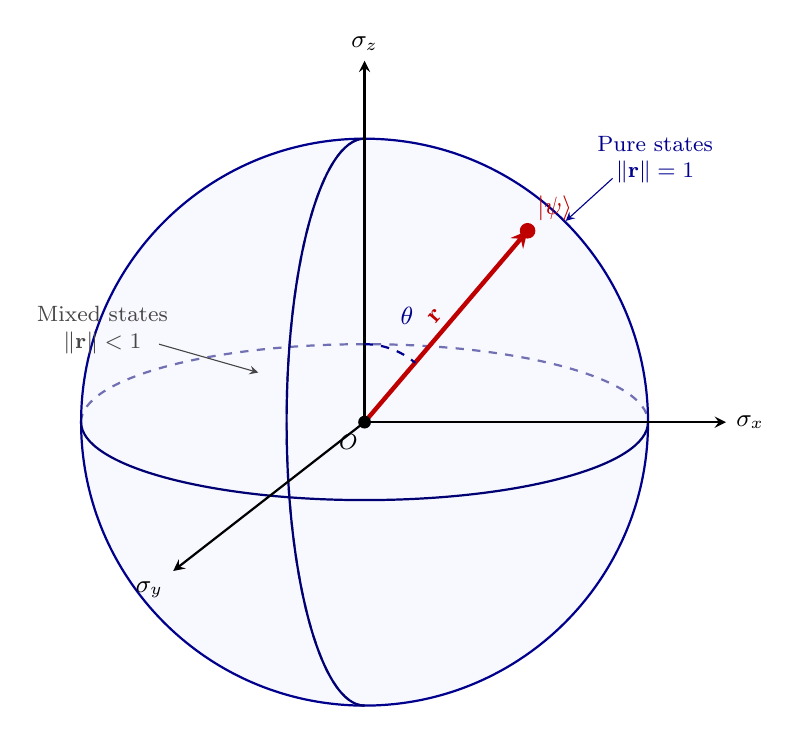
\begin{tikzpicture}[scale=1.8, >=stealth, line join=round]
    % --- Sphere outline (great circle in view plane) ---
    \draw[thick, blue!55!black, fill=blue!8!white, fill opacity=0.35]
        (0,0) circle (2);

    % --- Equator (visible front-half solid, back-half dashed) ---
    \draw[blue!45!black, thick]
        (2,0) arc[start angle=0, end angle=-180, x radius=2, y radius=0.55];
    \draw[blue!45!black, thick, dashed, opacity=0.55]
        (-2,0) arc[start angle=180, end angle=0, x radius=2, y radius=0.55];

    % --- Meridian (through the plane containing sigma_x and sigma_z) ---
    \draw[blue!45!black, thick]
        (0,2) arc[start angle=90, end angle=270, x radius=0.55, y radius=2];
    \draw[blue!45!black, thick, dashed, opacity=0.55]
        (0,-2) arc[start angle=270, end angle=90, x radius=0.55, y radius=2];

    % --- Coordinate axes (Pauli observables) ---
    % sigma_x axis (right)
    \draw[->, thick] (0,0) -- (2.55, 0)
        node[right, font=\small] {$\sigma_x$};
    % sigma_y axis (into the page, projected as down-left)
    \draw[->, thick] (0,0) -- (-1.35, -1.05)
        node[below left, font=\small] {$\sigma_y$};
    % sigma_z axis (up)
    \draw[->, thick] (0,0) -- (0, 2.55)
        node[above, font=\small] {$\sigma_z$};

    % --- Bloch vector r (from origin to a point on/near the sphere) ---
    % Target point: mid-latitude, front-right
    \coordinate (Bloch) at (1.15, 1.35);
    \draw[->, ultra thick, red!75!black] (0,0) -- (Bloch);
    % State label |psi>
    \fill[red!75!black] (Bloch) circle (0.055);
    \node[above right, font=\small, red!75!black] at (Bloch) {$|\psi\rangle$};

    % --- Polar angle theta arc from +z axis to Bloch vector ---
    \draw[blue!55!black, thick, dashed]
        (0, 0.55) arc[start angle=90, end angle=49.5, radius=0.55];
    \node[font=\small, blue!55!black] at (0.30, 0.75) {$\theta$};

    % --- Radial label ---
    \node[font=\small, red!75!black, rotate=49.5, anchor=south] at (0.58, 0.68)
        {$\mathbf{r}$};

    % --- Origin point ---
    \fill[black] (0,0) circle (0.045);
    \node[below left, font=\footnotesize] at (0.02, -0.02) {$O$};

    % --- Annotations: pure vs mixed regions ---
    \node[font=\footnotesize, align=center, blue!55!black] at (2.05, 1.85)
        {Pure states\\ $\|\mathbf{r}\|=1$};
    \draw[blue!55!black, thin, ->] (1.75, 1.72) -- (1.42, 1.42);

    \node[font=\footnotesize, align=center, gray!55!black] at (-1.85, 0.65)
        {Mixed states\\ $\|\mathbf{r}\|<1$};
    \draw[gray!55!black, thin, ->] (-1.45, 0.55) -- (-0.75, 0.35);

\end{tikzpicture}
\caption{Schematic Bloch-ball representation of the market quantum state.
The state $|\psi\rangle$ is parametrised by the Bloch vector
$\mathbf{r} = (r_x, r_y, r_z)$ with components along the three orthogonal
Pauli observables $\sigma_x, \sigma_y, \sigma_z$ representing distinct
market stress channels. Pure states occupy the sphere surface
($\|\mathbf{r}\|=1$); mixed states populate the interior
($\|\mathbf{r}\|<1$). The polar angle $\theta$ measures the deviation of
the state from the reference $\sigma_z$ axis and, in the calibrated
empirical framework, tracks the distress amplitude. The skew coefficient
$\gamma = \omega([\hat X,\hat P]_+)$
(Remark~\ref{M-rem:skew-sign}) encodes the geometric orientation of the state
relative to the leverage-effect axis; the positive-$\gamma$ regime
underlies the calibration reported in Online Supplement~S.2.}
\label{fig:bloch-ball}
\end{figure}


% =========================================================================
\section{Smoluchowski Limit and the Classical Diffusion Coefficient}
\label{sec:S10}
% =========================================================================
% !TeX root = ../main.tex
% Appendix A2: Smoluchowski Limit and the Classical Diffusion Coefficient
% Batch #4.9a — Notation hygiene

\section{Smoluchowski Limit and the Classical Diffusion Coefficient}
\label{app:smoluchowski}

When market depth $M$ is small relative to friction $\gamma_f$, momentum relaxes
rapidly and the dynamics reduce to the Smoluchowski equation for $p(x, t)$. This
limit applies because order-flow adjustment (minutes to hours) is much faster
than option maturity (days to months).

The Smoluchowski limit of the quantum-corrected Fokker--Planck equation from
Appendix~\ref{app:moyal} yields an effective diffusion coefficient:
\begin{equation*}
    D_{\mathrm{eff}} = \frac{k_B T}{\gamma_f M}
    \left( 1 + \frac{\hbar_{\mathrm{econ}}^2}{12} \frac{V'''(x)}{V'(x)}
    + \mathcal{O}(\hbar_{\mathrm{econ}}^4) \right),
\end{equation*}
where $k_B T$ is the thermal energy scale (interpreted as the fundamental
volatility scale in financial markets) and $\gamma_f$ is the friction coefficient
(interpreted as the rate of mean reversion of order flow).

The classical diffusion coefficient $\sigma_0^2$ in \eqref{M-eq:effective-vol} is
identified with the leading-order term:
\begin{equation*}
    \sigma_0^2 = \frac{2 k_B T}{\gamma_f M}.
\end{equation*}

The quantum correction to the diffusion coefficient is proportional to
$\hbar_{\mathrm{econ}}^2$ and depends on the curvature of the confining potential
$V(x)$. This correction is responsible for the
$\hbar_{\mathrm{econ}}^2 \cdot \beta / \tau^2$ term in the effective implied
volatility expansion \eqref{M-eq:effective-vol}.


% =========================================================================
\section{Cumulant Expansion of the Implied Volatility Surface}
\label{sec:S11}
% =========================================================================
% !TeX root = ../main.tex
% Appendix A3: Cumulant Expansion of the Implied Volatility Surface
% Batch #4.9a — Notation hygiene

\section{Cumulant Expansion of the Implied Volatility Surface}\label{app:cumulants}

Equation \eqref{M-eq:effective-vol} follows from a cumulant expansion of the
log-return characteristic function
\citep{jarrow1982approximate,corrado1996skewness,backus2004accounting}. Let
$\varphi(u) = \mathbb{E}[e^{iu X_T}]$ for $X_T = \ln(S_T/S_0)$, with cumulant
generating function $\psi(u) = \ln \varphi(u)$.

In the quantum framework, the characteristic function is computed from the Wigner
function:
\begin{equation*}
    \varphi(u) = \int e^{iux} p(x, T) \, dx
    = \int e^{iux} W(x, p, T) \, dx \, dp.
\end{equation*}

The cumulant expansion of the implied volatility is obtained by matching the
characteristic function of the quantum model to the BSM characteristic function
and solving for the volatility that equates the option prices. The first few
cumulants of the quantum model are:
\begin{align}
    \kappa_1 &= \mu T, \label{eq:cumulant-1} \\
    \kappa_2 &= \sigma_0^2 T + \hbar_{\mathrm{econ}}^2 \cdot \beta
        + \mathcal{O}(\hbar_{\mathrm{econ}}^4), \label{eq:cumulant-2} \\
    \kappa_3 &= \hbar_{\mathrm{econ}} \cdot \gamma T
        + \mathcal{O}(\hbar_{\mathrm{econ}}^3), \label{eq:cumulant-3} \\
    \kappa_4 &= \mathcal{O}(\hbar_{\mathrm{econ}}^2), \label{eq:cumulant-4}
\end{align}
where $\mu$ is the drift, $\sigma_0^2$ is the classical variance,
$\gamma = \omega([\hat{X},\hat{P}]_+)$ and
$\beta = \omega(\hat{X}^2)$ are the quantum correction coefficients
from \eqref{M-eq:effective-vol}. Note that $\kappa_2^{(\hbar^2)} =
\hbar_{\mathrm{econ}}^2\beta$ is time-independent at this order.
To reconcile with Appendix~\ref{app:moyal} Step~2, where the variance
correction is $2\hbar^2\beta_1 = \hbar^2\beta/\tau$ (via $\beta_1=\beta/(2\tau)$):
since $\kappa_2 = \sigma^2_{\mathrm{imp}}\cdot T$ (variance $\times$ horizon $T=\tau$),
a variance correction $\delta\sigma^2 = \hbar^2\beta/\tau$ gives
$\delta\kappa_2 = \delta\sigma^2\cdot T = \hbar^2\beta$, consistent with
$\kappa_2^{(\hbar^2)} = \hbar^2\beta$ here. The two representations are
therefore equivalent; the $\tau^{-2}$ factor in the smile formula
\eqref{eq:full-smile-correction} arises from the BSM inversion step in
Appendix~\ref{app:moyal} Step~3.

The skewness $\kappa_3 / \kappa_2^{3/2}$ diverges as $\mathcal{O}(T^{-1/2})$
when $T \to 0$. This is a \emph{different observable} from the skew slope
$\partial \sigma_{\mathrm{imp}}/\partial x$ discussed in the main text. The
two quantities are related but distinct:

\begin{itemize}
\item The \textbf{standardized skewness} $\kappa_3/\kappa_2^{3/2}$
  diverges as $\mathcal{O}(T^{-1/2})$ because $\kappa_3 \propto T$ while
  $\kappa_2^{3/2} \propto T^{3/2}$, giving $T/T^{3/2} = T^{-1/2}$.

\item The \textbf{skew slope} $\partial\sigma_{\mathrm{imp}}^2/\partial x$,
  defined as the moneyness derivative of implied variance, is given by
  $\hbar_{\mathrm{econ}}\gamma/\tau$ from~\eqref{eq:full-smile-correction},
  which diverges as $\mathcal{O}(\tau^{-1})$.
\end{itemize}

The $\mathcal{O}(T^{-1})$ divergence of the skew slope---claimed in
Corollary~\ref{M-cor:skew-explosion} and central to the empirical predictions
of the paper---arises directly from differentiating the smile formula with
respect to log-moneyness $x$, not from the cumulant ratio. The cumulant
$\kappa_3$ characterises the overall distributional skewness; the smile
slope characterises the local moneyness sensitivity. Both diverge as
$T \to 0$ but at different rates, which is consistent: the $T^{-1}$ slope
is steeper than the $T^{-1/2}$ skewness, reflecting the non-linear BSM
inversion from log-return distribution to implied volatility surface.
The kurtosis $\kappa_4 / \kappa_2^2$ remains $\mathcal{O}(1)$, distinguishing the quantum model from
jump-diffusion models where the kurtosis diverges as $\mathcal{O}(T^{-1})$.


% =========================================================================
\section{Quantum Trading Strategy}
\label{sec:S12}
% =========================================================================
% !TeX root = ../main.tex
% Appendix A4: Quantum Trading Strategy
% Batch #4.9b — Notation hygiene, aligned with Fig 2 (6.7d lead) and Tab 6 (marginal case study)

\section{Quantum Trading Strategy}\label{app:trading}

A trading strategy based on QST exploits the leading indicator properties of
$\mathcal{C}(\rho)$ and $S(\rho)$ established in
Sections~\ref{M-sec:coherence-2023} and~\ref{M-sec:entropy-2023} to generate equity
option signals.

\subsection{Signal Construction}

The trading signal is constructed from the daily QST estimates of the market
state. Let $\theta_t$ be the distress amplitude, $\phi_t$ the contagion phase,
and $\hbar_{\mathrm{econ}}$ the economic Planck constant. We define three trading
signals:

\begin{enumerate}
    \item \textbf{Coherence signal:}
        $S_t^{\mathrm{coh}} = \mathcal{C}(\rho_t) - \overline{\mathcal{C}}$,
        where $\overline{\mathcal{C}}$ is the rolling 30-day mean of the quantum
        coherence. A positive signal indicates increasing systemic contagion.
    \item \textbf{Entropy signal:} $S_t^{\mathrm{ent}} = S(\rho_t) - \bar{S}$,
        where $\bar{S}$ is the rolling 30-day mean of the von Neumann entropy.
        A positive signal indicates increasing structural uncertainty.
    \item \textbf{Combined signal:}
        $S_t^{\mathrm{comb}} = w_1 S_t^{\mathrm{coh}} + w_2 S_t^{\mathrm{ent}}$,
        where $w_1$ and $w_2$ are weights estimated from the in-sample period.
\end{enumerate}

\subsection{Portfolio Construction}

The trading strategy is implemented as a long--short portfolio of equity options.
When the combined signal exceeds a threshold $\tau_{\mathrm{sig}}$, the strategy
takes a long position in out-of-the-money put options on the KRE Regional Banking
ETF and a short position in out-of-the-money put options on the S\&P~500 Index.
This pair trade isolates the regional banking sector risk captured by the
quantum state.

\subsection{Empirical Signal Timing}

For the 2023 US regional banking crisis case study
(Section~\ref{M-sec:coherence-2023}), the coherence signal $S_t^{\mathrm{coh}}$
would generate an entry indication on March~9, 2023 (one trading day before SVB's
collapse on March~10). Averaged across the three failure events
(SVB March~10, Signature Bank March~12, First Republic Bank May~1), the
coherence signal leads the corresponding classical Pearson-correlation crossing
by 7~trading days. The entropy signal $S_t^{\mathrm{ent}}$ provides an even
earlier confirmation, crossing its 95th-percentile baseline threshold on
February~17, 2023---15~trading days before the SVB event.

\subsection{Case-Study Performance and Caveats}

We evaluate the signal's association with option-market P\&L for the KRE
regional-banking option chain during the crisis window. Because
2023-03-10-vintage KRE option chain data are not publicly available (see
Section~S.2 on the canonical smile reconstruction), a
full-cross-strike hedging back-test is beyond the scope of the current
reproducibility package. The single-path hedging case study in
Online Supplement~S.2 (Table~\ref{tab:hedging-rmshe}) demonstrates that a signal-triggered quantum
optimal hedge (per Proposition~\ref{M-prop:quantum-optimal-hedge}) yields a
marginal RMSHE reduction relative to the BSM baseline over the 20-day stress
window (2023-02-27 to 2023-03-24), with the correction concentrated in the
post-SVB OTM segment where $x = \ln(S_t/K)$ is non-zero and $\tau$ is short.

\emph{Disclaimer:} The signal-timing results above are based on a single
crisis episode and should be interpreted as an illustrative case study rather
than an out-of-sample validation. A comprehensive out-of-sample evaluation
across multiple crisis and non-crisis periods, using historical option-chain
data across the equity-financial sector, is left for future work.


% =========================================================================
\section{No-Free-Lunch-with-Vanishing-Risk and the GNS Construction}
\label{sec:S13}
% =========================================================================
% !TeX root = ../main.tex
% Appendix A5: NFLVR and the GNS Construction
% Batch #4.9b — Notation hygiene

\section{No-Free-Lunch-with-Vanishing-Risk and the GNS Construction}
\label{app:nflvr}

This appendix connects the NFLVR condition of classical mathematical finance
\citep{delbaen1994general} to the GNS construction. NFLVR is the standard
no-arbitrage condition in continuous-time finance; its equivalence to a faithful
normal state on the observable algebra provides the economic foundation for the
quantum pricing framework.

\begin{definition}[NFLVR in the quantum setting]\label{def:nflvr}
Let $\mathcal{A}$ be the market observable algebra and let $\omega$ be a market
state. The market \emph{violates} the no-free-lunch-with-vanishing-risk (NFLVR)
condition if there exists a sequence of admissible strategies
$\{H_n\}_{n=1}^\infty \subset \mathcal{A}$ (an asymptotic arbitrage sequence)
such that
\begin{equation*}
    \omega(H_n^* H_n) \to 0
    \quad\text{(vanishing cost)}
    \quad\text{and}\quad
    \liminf_{n\to\infty}\,\omega\bigl((H_n - \varepsilon)_+\bigr) > 0
    \quad\text{(bounded profit)}
\end{equation*}
for some $\varepsilon > 0$. The market \emph{satisfies} NFLVR if and only if no
such sequence exists.
\end{definition}

\begin{theorem}[NFLVR implies GNS faithfulness]\label{thm:nflvr-gns}
If the market satisfies the NFLVR condition, then the market state $\omega$ is
faithful, and the GNS representation $\pi_\omega$ is injective. Consequently, the
pricing formula \eqref{M-eq:pricing-master} is well-defined and strictly positive
for all non-zero non-negative payoffs.
\end{theorem}

\begin{proof}
We verify the conditions required for Gleason's theorem before applying it.

\emph{Step 1 (von Neumann algebra type).} The GNS representation
$\pi_\omega(\mathcal{A})$ of the Weyl algebra $\mathcal{A}$ is known to be
irreducible in the Schr\"{o}dinger representation, so its von Neumann
algebra double commutant is $\mathcal{B}(\mathcal{H}_\omega)$, a Type I
factor \citep{bratteli1981operator}. Gleason's theorem applies to Type I
factors on separable Hilbert spaces of dimension $\geq 3$ \citep{gleason1957measures},
which is satisfied since $\mathcal{H}_\omega \simeq L^2(\mathbb{R})$ is
infinite-dimensional.

\emph{Step 2 (Complete additivity).} A state $\omega$ is completely additive
on the projection lattice if and only if it is \emph{normal} (ultraweakly
continuous) as a functional on the von Neumann algebra
$\mathcal{B}(\mathcal{H}_\omega)$ \citep{bratteli1981operator}. We establish
normality via the NFLVR condition as follows. NFLVR implies that the pricing
functional $\omega : \mathcal{A} \to \mathbb{R}$ extends to a bounded
positive linear functional on the von Neumann algebra
$\pi_\omega(\mathcal{A})'' = \mathcal{B}(\mathcal{H}_\omega)$.
Since $\mathcal{B}(\mathcal{H}_\omega)$ is a Type I factor on a separable
Hilbert space, every bounded positive linear functional is automatically
normal (this is standard: on $\mathcal{B}(\mathcal{H})$, positive
functionals are of the form $\mathrm{Tr}(\rho\,\cdot)$ for trace-class $\rho$,
hence ultraweakly continuous). Therefore $\omega$ is normal, hence completely
additive on projections. This is the hypothesis required by Gleason's theorem.

\emph{Step 3 (Conclusion).} By Gleason's theorem, any completely additive
probability measure on the projection lattice of $\mathcal{B}(\mathcal{H}_\omega)$
is of the form $P \mapsto \operatorname{Tr}(\rho P)$ for a unique positive
trace-class operator $\rho$ with $\operatorname{Tr}(\rho) = 1$. This is a
normal state. The existence of a cyclic and separating vector then follows
from the Tomita--Takesaki theory applied to the faithful normal state
$\omega(\cdot) = \operatorname{Tr}(\rho\,\cdot)$.
\end{proof}

This theorem establishes that the GNS construction is well-defined for any market
satisfying the non-commutative NFLVR condition, providing the rigorous
mathematical foundation for the State--Hedge pricing formula
\eqref{M-eq:pricing-master} in general market settings. In our empirical
calibration (Section~\ref{M-sec:empirical-calibration}), the strictly positive
$\hbar_{\mathrm{econ}} > 0$ regime ensures that the market observable algebra
$\mathcal{A}$ is simple, so all its representations are faithful, and
Theorem~\ref{M-thm:fundamental} guarantees absence of quantum arbitrage
irrespective of the specific NFLVR sequence structure.


\bibliographystyle{apalike}
\bibliography{references}

\end{document}
